\section{Woche 18 - CVSS Calculator Web UI} \label{sec:bericht-wo-18}

% 2024-01-15 bis 2024-01-19

\lweekdaymarginpar{\weekdayMondayShort, \weekdayTuesdayShort}

Den Beginn der Woche verbrache ich damit, die Implementierung von CVSS:4.0 abzuschließen.
Im Vergleich zur offiziellen JavaScript-Referenzimplementierung\footnote{\url{https://github.com/RedHatProductSecurity/cvss-v4-calculator/blob/main/app.js}} ist mein Ansatz in TypeScript deutlich objektorientierter und meiner Meinung nach übersichtlicher.
Dazu habe ich einen eher ungewöhnlichen Ansatz gewählt:
ich übertrug die Java-Klassen erst einmal 1:1 in TypeScript und passte sie dann Stück für Stück an die Zielsprache an.
Zirkuläre Referenzen löste durch mit madge\footnote{\url{https://www.npmjs.com/package/madge}} erzeugten Visualisierungen.

\sweekdaymarginpar{\weekdayWednesdayShort\ - \weekdayFridayShort}

Nachdem alle Tests bestanden waren, implementierte ich das Web-Interface mit Bootstrap\footnote{\url{https://getbootstrap.com/}} und ChartJs.
Ich erstellte eine HTML-Struktur und entsprechendes JavaScript, um mit der CVSS-Bibliothek oder der NVD-API zu interagieren.
Nach der Basisfunktionalität verbesserte ich das UI, fügte Lizenzinformationen hinzu, räumte die Bibliothek auf und erstellte Dokumentation.
Das Ergebnis kann in Abb. \ref{fig:metaeffekt-cvss-calculator-ui} gesehen werden.
Das Projekt veröffentlichte ich auf GitHub\footnote{\url{https://github.com/org-metaeffekt/metaeffekt-universal-cvss-calculator}} und teilte es auf LinkedIn\footnote{\url{https://www.linkedin.com/feed/update/urn:li:activity:7151175714694729728/}}.
Das Feedback von unseren Kunden war sehr positiv, mit vielen interessanten Verbesserungsvorschlägen.

\begin{figure}[htbp] % here, top, bottom, separate page
    \centering
    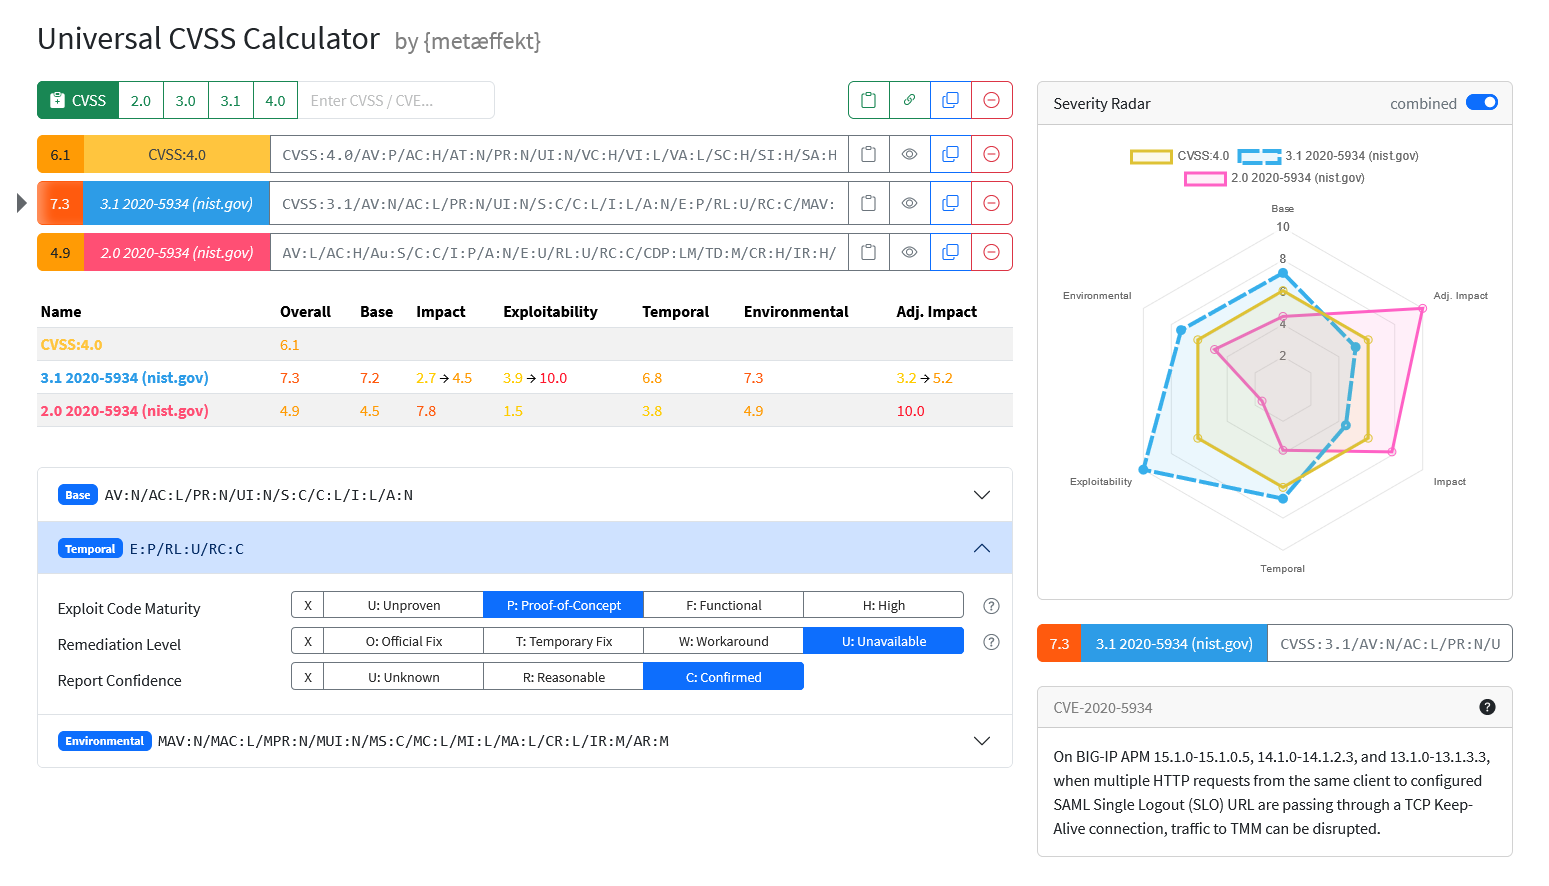
\includegraphics[width=0.8\textwidth, keepaspectratio]{res/img/metaeffekt-cvss-calculator-ui}
    \caption{Der {\metaeffekt} Universal CVSS-Rechner}
    \label{fig:metaeffekt-cvss-calculator-ui}
\end{figure}

Von Shane Coughlan, OpenChain General Manager und ein Referent des Open Source Forum der bitkom, haben wir freundlicherweise folgendes Zitat zu unserem Rechner erhalten:

\begin{quote}
    \textit{\qt{Contextualizing security threats is as important as identifying their existence,” says Shane Coughlan, OpenChain General Manager. “The emergence of open source tools to visualize this is a key part of ensuring the supply chain can plan ahead and action responses. We are delighted to see the work by Metaeffekt, an official OpenChain Partner, in the domain. It aligns well with OpenChain ISO/IEC 18974, the international standard for open source security assurance.}}
\end{quote}
